\section{Jakub Halfar}
\label{sec:jakub_halfar}

\subsection{Mathematics}
\subsubsection{Nicomachus's theorem}
\underline{\textbf{Nicomachus's theorem}} (see proof on Figure~\ref{fig:nicomachus_proof}) states that the sum of the first $n$ cubes equals the square of the sum of the first $n$ natural numbers. In mathematical notation, that is:
\[
1^3 + 2^3 + 3^3 + \dots + n^3 = (1 + 2 + 3 + \dots + n)^2
\]
Using the capital sigma notation, one can write this succinctly as:
\[
\sum_{k=1}^n k^3 = \left( \sum_{k=1}^n k \right)^2
\]
The sum of the first $n$ natural numbers is often denoted as the $n$-th triangular number $T_n$, because it represents the number of objects needed to form an equilateral triangle with the base made of $n$ objects and each subsequent layer made of exactly one object less.
\[
\sum_{k=1}^n k^3 = T_{n}^2
\]
This theorem has a very elegant \textit{proof without words}, which uses a clever rearrangement of objects.
\begin{figure}[htbp] % Image placement priority: h (here), t (top), b (bottom), p (page)
    \centering
    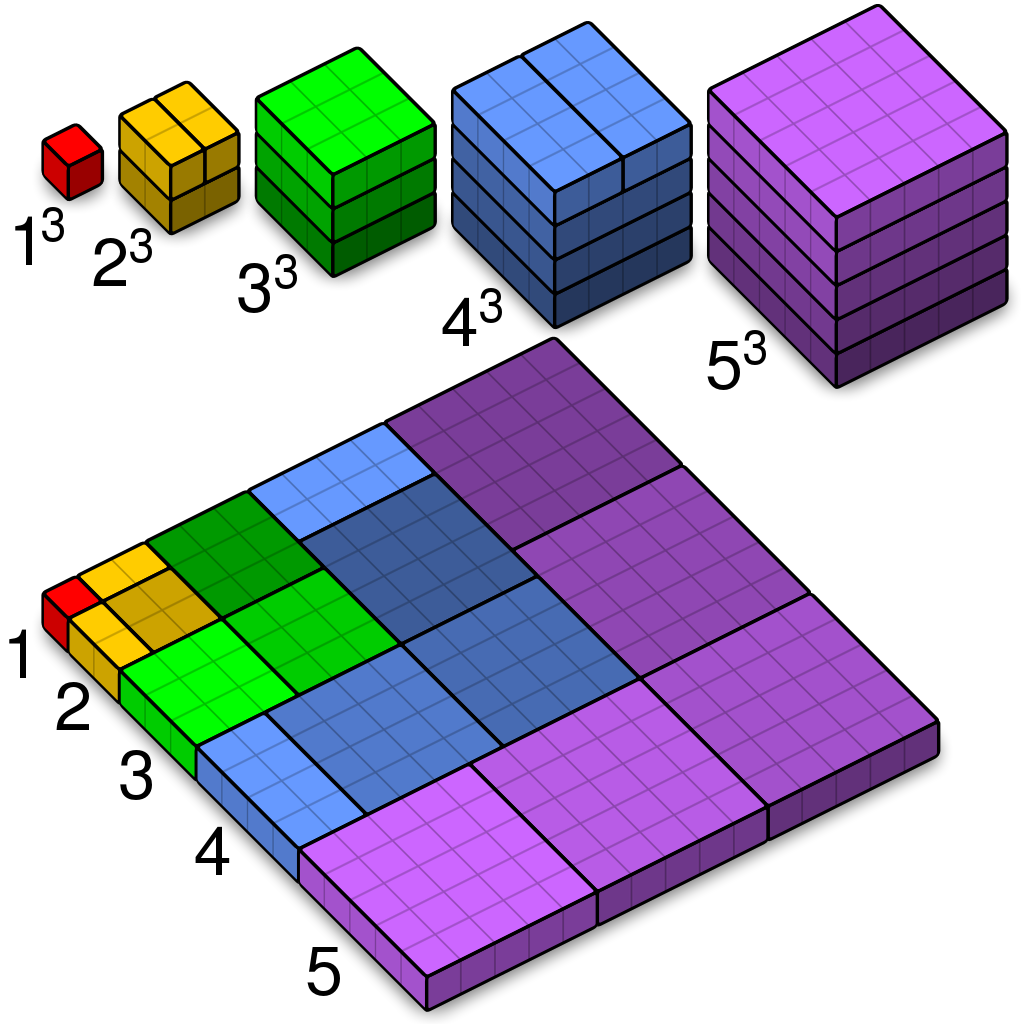
\includegraphics[width=0.45\textwidth]{nicomachus_theorem.png} % Adjusted the image width
    \caption{Proof of the Nicomachus's theorem}
    \label{fig:nicomachus_proof}
\end{figure}

\subsubsection{Constants}
Mathematics is rich in different constants, which show up in very unexpected places and formulas. Table~\ref{tab:math_constants} lists some of the lesser-known ones, which are still very important and are some of my favorite.
\begin{table}[htbp]
\centering
\begin{adjustbox}{width=\textwidth}
\begin{tabular}{|Sc|Sc|Sc|Sc|}
\hline
\rowcolor{LimeGreen}
\textbf{Name} &
  \thead{Symbol} &
  \thead{Decimal \\ expansion} &
  \thead{Formula} \\ \hline
\makecell{Euler–Mascheroni \\ constant} &
  $\gamma$ &
  $0.57721\dots$ &
  $\displaystyle\gamma = \lim_{n\to\infty} \left(-\ln\left(n\right) + \sum_{k=1}^n \frac{1}{k}\right)$ \\ \hline
Dottie number &
  $D$ &
  $0.73908\dots$ &
  $\displaystyle\cos D = D$ \\ \hline
Catalan's constant &
  $G$ &
  $0.91596\dots$ &
  $G = \displaystyle\sum_{n=0}^\infty \frac{(-1)^n}{(2n+1)^2}$ \\ \hline
Omega constant &
  $\Omega$ &
  $0.56714\dots$ &
  $\displaystyle\Omega e^\Omega = 1$ \\ \hline
\makecell{Universal parabolic \\ constant} &
  $P$ &
  $2.29558\dots$ &
  $\displaystyle P = \ln\left(1+\sqrt{2}\right) + \sqrt{2}$ \\ \hline
Conway's constant &
  $\lambda$ &
  $1.30357\dots$ &
  \makecell{$\displaystyle\lambda = \lim_{n\to\infty} \frac{L_{n+1}}{L_n}$ \\ where $L_n$ is the number of \\ digits in the $n$-th \\ \href{https://en.wikipedia.org/wiki/Look-and-say_sequence}{look-and-say} sequence member } \\ \hline
\makecell{Reciprocal Fibonacci \\ constant} &
  $\psi$ &
  $3.35988\dots$ &
  \makecell{$\displaystyle\psi = \sum_{k=1}^\infty \frac{1}{F_k}$ \\ where $F_k$ is the $k$-th \\ Fibonacci number \\ ($F_1 = 1$, $F_2 = 1$, $F_n = F_{n-1} + F_{n-2}$)} \\ \hline
\end{tabular}
\end{adjustbox}
\caption{A few interesting mathematical constants}
\label{tab:math_constants}
\end{table}
\newpage

\subsection{Computer science}
\subsubsection{Top 3 best operating systems, but ranked alphabetically:}
\begin{enumerate}
    \item Linux
    \item macOS
    \item Windows
\end{enumerate}

\subsubsection{\texttt{YAML} meaning}
\hypertarget{sssec:yaml}{}
Did you know that \hyperlink{sssec:yaml}{\texttt{YAML}} stands for:
\begin{itemize}[label=$\star$]
    \item \hyperlink{sssec:yaml}{\texttt{YAML}}
    \item Ain't
    \item Markup
    \item Language
\end{itemize}

\noindent
If you don't know what \hyperlink{sssec:yaml}{\texttt{YAML}} means, see the \hyperlink{sssec:yaml}{\texttt{YAML}} meaning.

\subsubsection{How to exit Vim?}
This is such a \textbf{tough} question that I had to ask \textit{Artificial Intelligence} to help us accomplish this task in \underline{as few steps as possible}.
\vspace{12pt}

\centerline{\textbf{\textit{"Escaping Vim: A Tale of Text Editing Adventures"}}}
\vspace{4pt}
Once upon a time in the realm of \textbf{text editing}, there was a mysterious land known as \textit{Vim}. To traverse this land, one had to navigate through its various \textbf{modes} and \textbf{commands}, each offering a unique passage to explore.

The journey began in the serene land of \textbf{Normal Mode}, the default realm when one first entered a file in \textit{Vim}. To exit \textbf{Normal Mode}, travelers would press the trusty \textbf{"Esc"} key, a signal to prepare for departure. They would then whisper the command \textbf{":q"} to kindly request \textit{Vim} to allow them to quit or \textbf{":q!"} to make a \underline{forceful exit}, casting aside unsaved changes like forgotten dreams. If one cherished their written adventures and desired to save them for posterity, they would craft the command \textbf{":wq"} or the elegant \textbf{":w"} to save the manuscript \underline{without bidding farewell}. And when the need was to escape \textit{Vim} in haste, without pausing to save a single word, they would call upon the magical \textbf{":q!"} command in \textbf{Normal Mode}.

But \textit{Vim} was no ordinary land; it was a tapestry woven with a rich array of commands and features, a terrain begging to be explored. The \textbf{"Esc"} key served as a trusty guide, guiding adventurers between the distinct modes, while the \textbf{":"} key was the key to \textbf{unlocking \emph{command mode}}, a portal where one could issue instructions to the enigmatic world of text editing. Each command chosen was akin to a decision on their journey, leaving an indelible mark on the unfolding narrative of their text adventure.